%\documentclass[authoryear,5p]{elsarticle}
%\documentclass[authoryear,review,11pt]{elsarticle}
\documentclass[11pt]{elsarticle}
\bibliographystyle{elsarticle-harv}
\usepackage{graphicx}
\usepackage{amsmath,amsfonts}
\usepackage{lineno}
\linenumbers
\usepackage{subfigure}
\usepackage[pdftex]{color}
\definecolor{darkblue}{rgb}{0,0,0.5}
\definecolor{darkgreen}{rgb}{0,0.5,0}
%\usepackage[pdftex, colorlinks, citecolor=darkblue,linkcolor=darkgreen]{hyperref}
\usepackage[pdftex, colorlinks]{hyperref}
\textwidth 6.75in
\oddsidemargin -0.15in
\evensidemargin -0.15in
\textheight 9in
\topmargin -0.5in
\newcommand{\ud}{\mathrm{d}}
\newcommand{\E}{\mathrm{E}}
\newcommand{\C}{\mathrm{Cov}}
\newcommand{\V}{\mathrm{Var}}


%\graphicspath{{/home/cboettig/Documents/ucdavis/research/phylotrees/images/}}

\journal{a Letter to \emph{Ecology Letters}, Supplementary Information} 
\begin{document}
%\begin{frontmatter}
%  \title{  }
%  \author[cpb]{Carl Boettiger\corref{cor1}}
%  \author[alan]{Alan Hastings}
%  \ead{cboettig@ucdavis.edu}
%  \cortext[cor1]{Corresponding author.}
%  \address[cpb]{Center for Population Biology, University of California, Davis, United States}
%  \address[esp]{Department of Environmental Science and Policy, University of California, Davis, United States}
%\end{frontmatter}
%
\appendix
\renewcommand*\thefigure{S\arabic{figure}}
\renewcommand*\theequation{S\arabic{equation}}
\section{Comparing Models}\label{Cox}
Likelihood methods form the basis of much of modern statistics, in both Frequentist and Bayesian paradigms.  
The ability evaluate likelihoods directly by computation has made it possible to treat cases that do not conform to traditional assumptions more directly.
The basis of likelihood comparisons has its roots in the Neyman-Pearson Lemma, 
which essentially asserts that comparing likelihoods is the most powerful test
of a choice between two hypotheses~\citep{Neyman1933}, which motivates
tests from the simple likelihood ratio test up through modern model adequacy methods.

The hypotheses considered here are more challenging then the original lemma, as they are composite in nature:
they specify two model forms (stable and changing stability)
but with model parameters that must be first estimated from the data.
Comparing models whose parameters have been estimated by maximum likelihood is first treated by~\citet{Cox1961, Cox1962},
and has since been developed in this simulation estimation of the null distribution~\citep{McLachlan1987}, by parametric bootstrap estimate~\citep{Efron1987}.  
Cox's $\delta$ statistic is simply the difference between the log likelihoods of these maximum likelihood estimates, defined as follows.

Let $L_0$ be the likelihood function for model 0, 
let $\theta_0 = \arg \max \theta_0 \in \Omega_0$, ($L_0 (\theta_0 |X)$) 
be the maximum likelihood estimator for $\theta_0$ given $X$, and let $L_0 = L_0 (\theta_0 |X)$; 
and define $L_1$, $\theta_1$, $L_1$ similarly for model 1. 
The statistic we will use is $\delta$, 
defined to be twice the difference in log likelihood of observing the data under the two MLE models,
$\delta = -2 (\log L_0 - \log L_1 )$.  
This approach has been applied to the problem of model adequacy~\citep{Goldman1993} and model choice~\citep{Huelsenbeck1996} in other contexts.  
We have extended the approach by generating the test distribution as well as a null distribution of the statistic $\delta$ in order to compute ROC curves.  
Our results have shown that $\delta$ tends to result in lower error rates than $\tau$, the measure of increase in a summary statistic.  


\pagebreak

\section{On a hypothesis-testing framework}\label{Dakos}
It is possible to frame the question of sensitivity, reliability, and adequate data in the language of hypothesis testing. As this introduces the unnecessary nuisance parameter, the statistical significance criterion, it is not presented in the text.  In the hypothesis testing framework, a false positive is a Type I error, which is defined relative to some arbitrary statistical significance criterion, most commonly 0.05.  By changing this criterion, one can increase or decrease the probability of the Type I error at the cost of decreasing or increasing the Type II error, also defined relative to this criterion.  

The work by~\citet{Dakos2008} is one of the few commendable examples that attempts a careful quantification of the statistical significance of the increase observed in the indicator statistic (autocorrelation in this case).  We note that the $p$-values presented in the main text of that work are based on parametric assumptions not met by the data -- the autocorrelation is computed by a sliding window, and the points are part of a time series, both conditions that do not satisfy the null hypothesis that $x$ and $y$ are independent, which is used in approximating a normal distribution of $\tau$ values.  For this reason we generate the null distribution directly from the model as outlined above.   The rather different $p$ values presented in appendix of~\citet{Dakos2008}, Table S3 are constructed with more reasonable null hypotheses (in particular, H$_0$-2 and H$_0$-3 are very similar to our stable system, though H$_0$-1 has lost the correlation structure expected in any time-series).  The plots in Fig. 3 confirm our finding that almost any value of Kendall's $\tau$ is possible under the null hypothesis, and the $p$-values in table S3 show that the detection method is not significant in any of the time series that had fewer than 400 points.  Our approach replicate these findings for the $\tau$-statistic.  We were glad to find that our likelihood-based approach does not have this difficulty, easily identifying the warning signal in these shorter time series, while also reliably avoiding false alarms.  

The approach taken by~\citet{Dakos2008} does not present the corresponding analysis of power or Type II error.  As statistical significance could be achieved with a method that selects less than one in every twenty data sets at random, it is impossible to know whether the approach is actually detecting a signal or simply a random pattern in the noise without a test of power.  Fig. S3, highlights the importance of so doing -- the null distribution is almost uniform across all possible values of $\tau$.  The distribution of $\tau$ under the test distribution will not be able to avoid at least some overlap on this bounded domain.  The reality is worse, we find it overlaps almost completely.  We were glad to see that in estimating the distribution of $\tau$ for very large data sets, it does tighten around zero, while the distribution expected under a true positive condenses around more positive values, indicating that there is at least some discriminative ability in the test. 

The essential features of these overlapping distributions are easily captured in the ROC curves, which provides a natural language to discuss the issues of uncertainty -- such as ``accepting a higher false-alarm rate in order to avoid a catastrophic shift'' rather than ``using a more liberal threshold for $p$-values in order to avoid costly Type II error.''  



\section{R package tutorial}\label{R}
We provide an R package with simple implementation of the methods described here.  The package is available from: \href{https://github.com/cboettig/warningsignals/archives/master}{https://github.com/cboettig/warningsignals/archives/master}, where it will be actively maintained and developed.  The package takes an R time-series object (or, for unevenly spaced data -- a matrix or data-frame with sample times in the first column and observations in the second) as input and performs the likelihood-based analysis:

\begin{verbatim}
> require(warningsignals)
>
> # Load a sample dataset
> data(glaciationIII)
>
> # Fit constant (OU) model and a stability-loss model (LSN);
> models <- fit_models(glaciationIII, 'LSN')
>
> results <- montecarlotest(models$const, models$timedep, n=2000, cpu=16)
> plot(results)
\end{verbatim}

The package also performs the computationally faster but less powerful summary-statistic tests, computes the resulting distributions under the different hypotheses and the corresponding ROC curves.  The package allows a variety of correlation tests (Pearson's, Kendall's, Spearman's) as the measure of increase, and a variety of summary statistics (variance, autocorrelation, skew, coefficient of variation).  Copies of data used in the paper are provided as examples.  The Monte Carlo methods can take advantage of multiple core processors or clusters by specifying the number of CPUs in the function argument.   Full documentation of functions and data are provided in the package, as well as example scripts which replicate the analyses presented in the paper.   

 \section{Distributions of the indicator statistic}
The ROC curves are generated from distributions of the measure of increase, $\tau$, in a warning statistic (variance, autocorrelation, etc.) or the likelihood ratio $\delta$ from the likelihood approach.  The value of the statistic observed in the original data is indicated by a black triangle. Deciding whether or not this observed value indicates an early warning or not depends on the location of the threshold.  Thresholds involving larger values of $\tau$ or $\delta$ will generally involve fewer false alarms, but also catch fewer of the true positives.  The large overlap between the distribution under the stable model (blue) and the deteriorating stability system (red) indicates how difficult it can be for such statistics to discriminate between these alternatives.  The nature of this trade-off is illustrated by the ROC curve, which can therefore be helpful in selecting the threshold for a particular statistic.  


\begin{figure}[ht]
  \begin{center}
    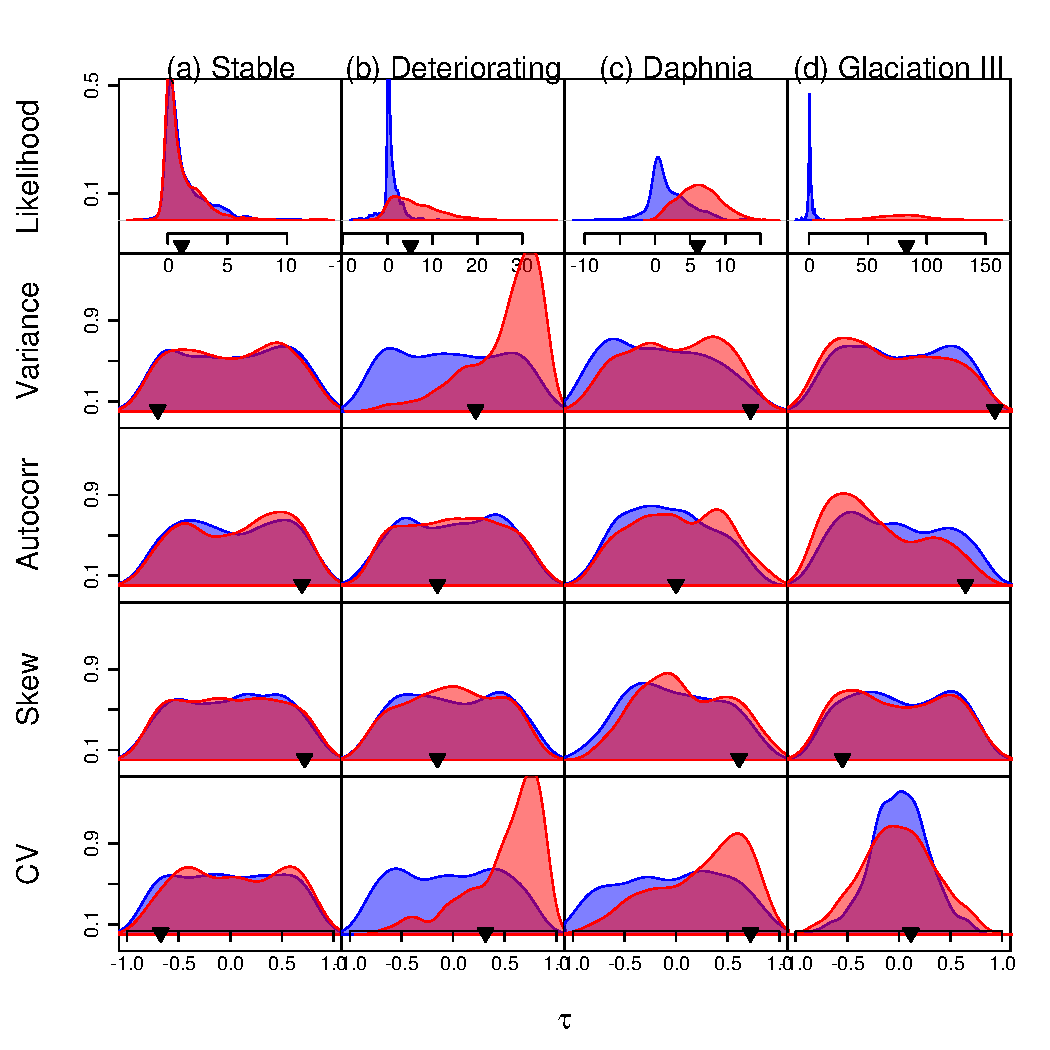
\includegraphics{FigS1.pdf}
  \end{center}
  \caption{Distribution of the indicator statistics corresponding to the ROC curves in Fig. 3, main text. As in Fig. 1, the expected distribution of the statistic under the null hypothesis of a stable system is shown in blue, while the distribution under the estimated deteriorating stability system is shown in red.  The value of the test statistic ($\delta$ in Likelihood, top row, otherwise $\tau$), observed in the original time-series is indicated by the black triangle. Distributions are produced from a Gaussian kernel density estimate from 500 replicates, as described in Methods.}
  \label{fig:S1}
\end{figure}

\begin{figure}[ht]
  \begin{center}
    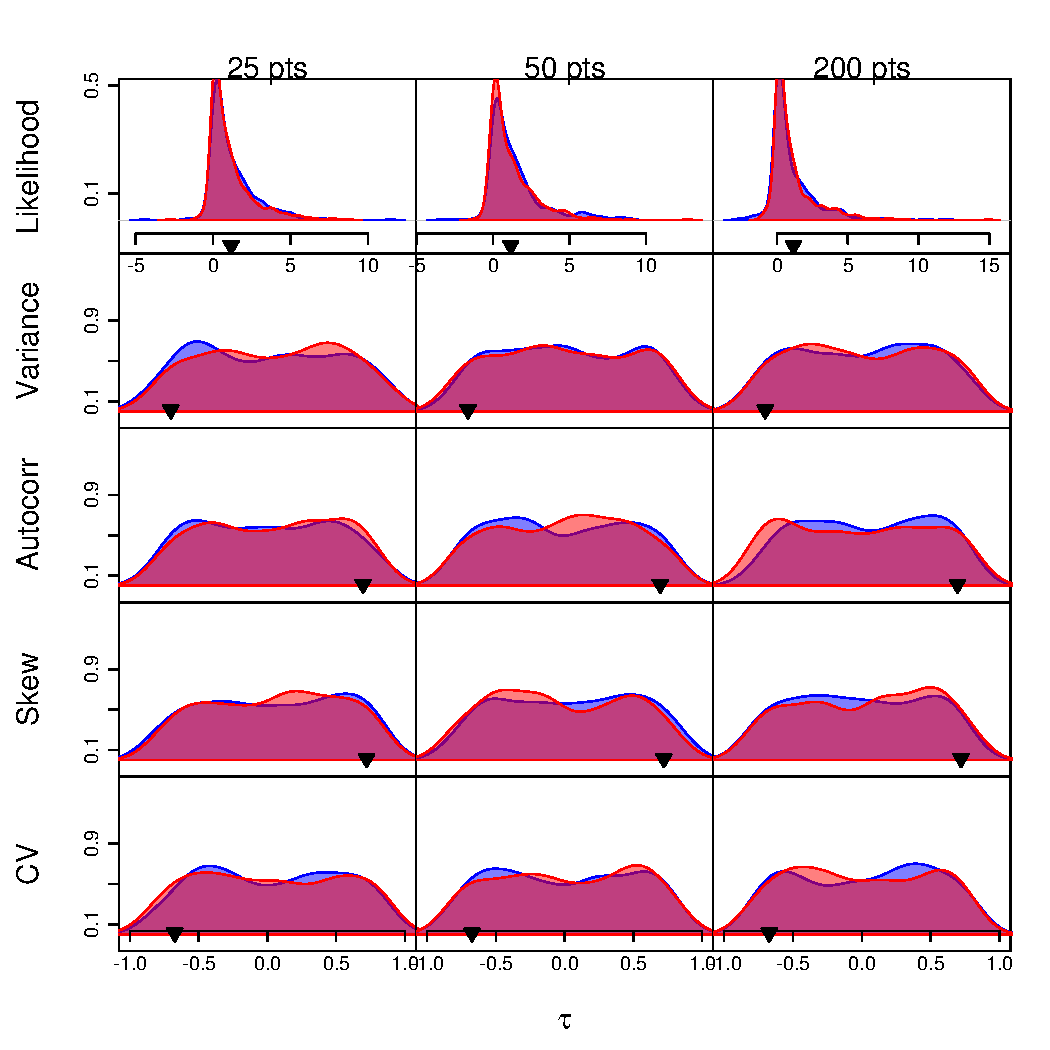
\includegraphics{FigS2.pdf}
  \end{center}
  \caption{Distributions of the indicator statistic as the sampling effort increases in the simulated data of a stable system, corresponding to the first column of Fig. 4, main text.  Distributions as described in caption of Fig~\ref{fig:S1}.}
  \label{fig:S2}
\end{figure}

\begin{figure}[ht]
  \begin{center}
    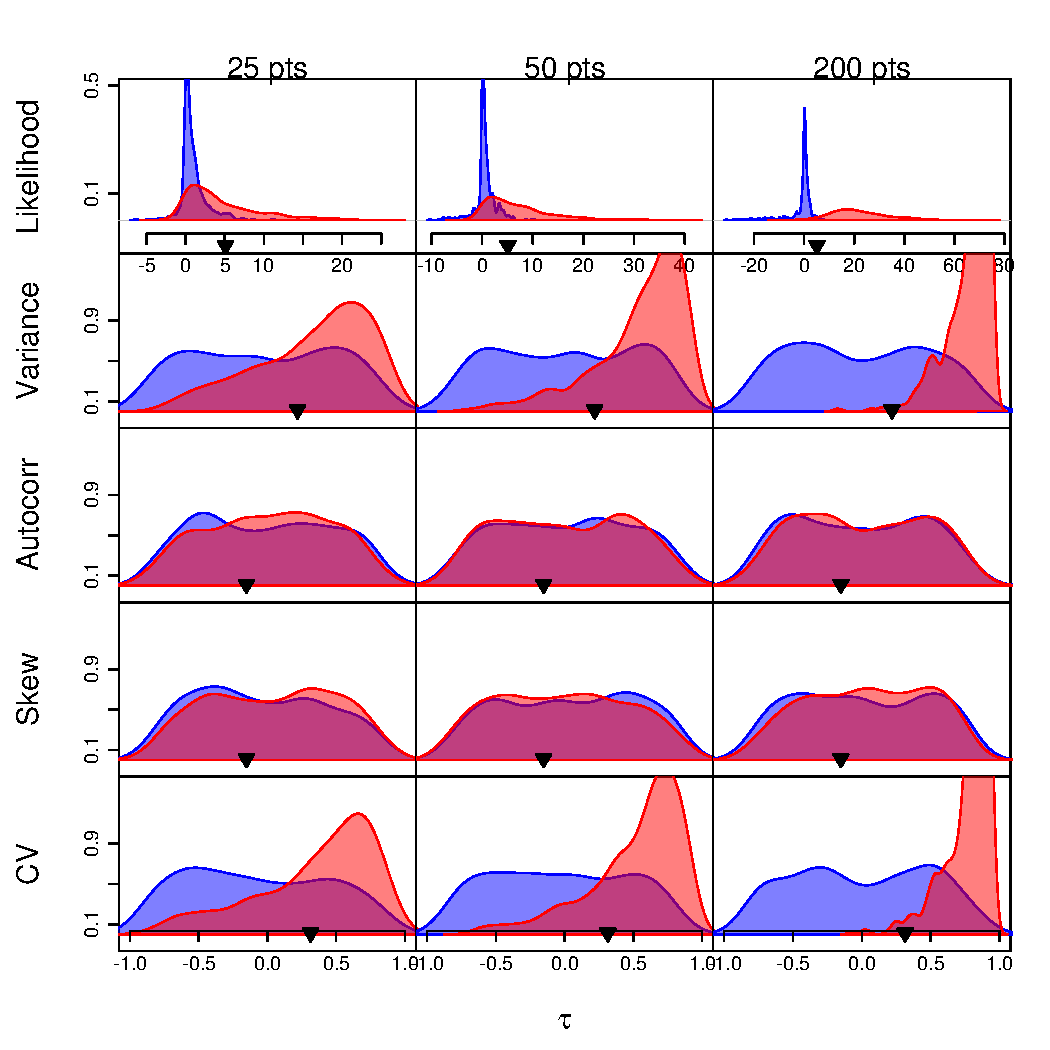
\includegraphics{FigS3.pdf}
  \end{center}
  \caption{Distributions of the indicator statistic as the sampling effort increases in the simulated data of a system under deteriorating stability, corresponding to the second column of Fig. 4, main text.  Distributions as described in caption of Fig~\ref{fig:S2}.}
  \label{fig:S3}
\end{figure}




\begin{figure}[ht]
  \begin{center}
    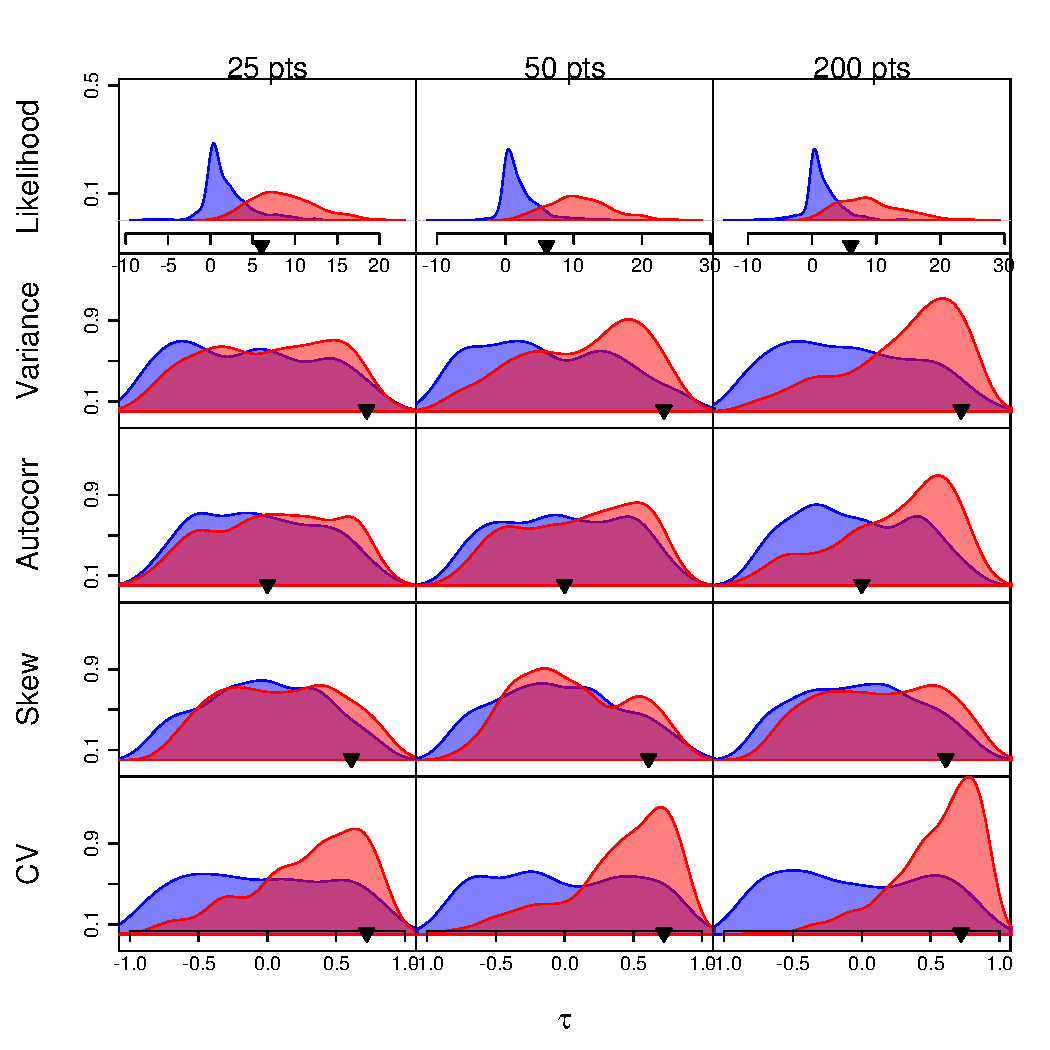
\includegraphics{FigS4.pdf}
  \end{center}
  \caption{Distributions of the indicator statistic as the sampling effort increases in the \emph{Daphnia} data, corresponding to the third column of Fig. 4, main text.  Distributions as described in caption of Fig~\ref{fig:S1}.}
  \label{fig:S4}
\end{figure}


\begin{figure}[ht]
  \begin{center}
    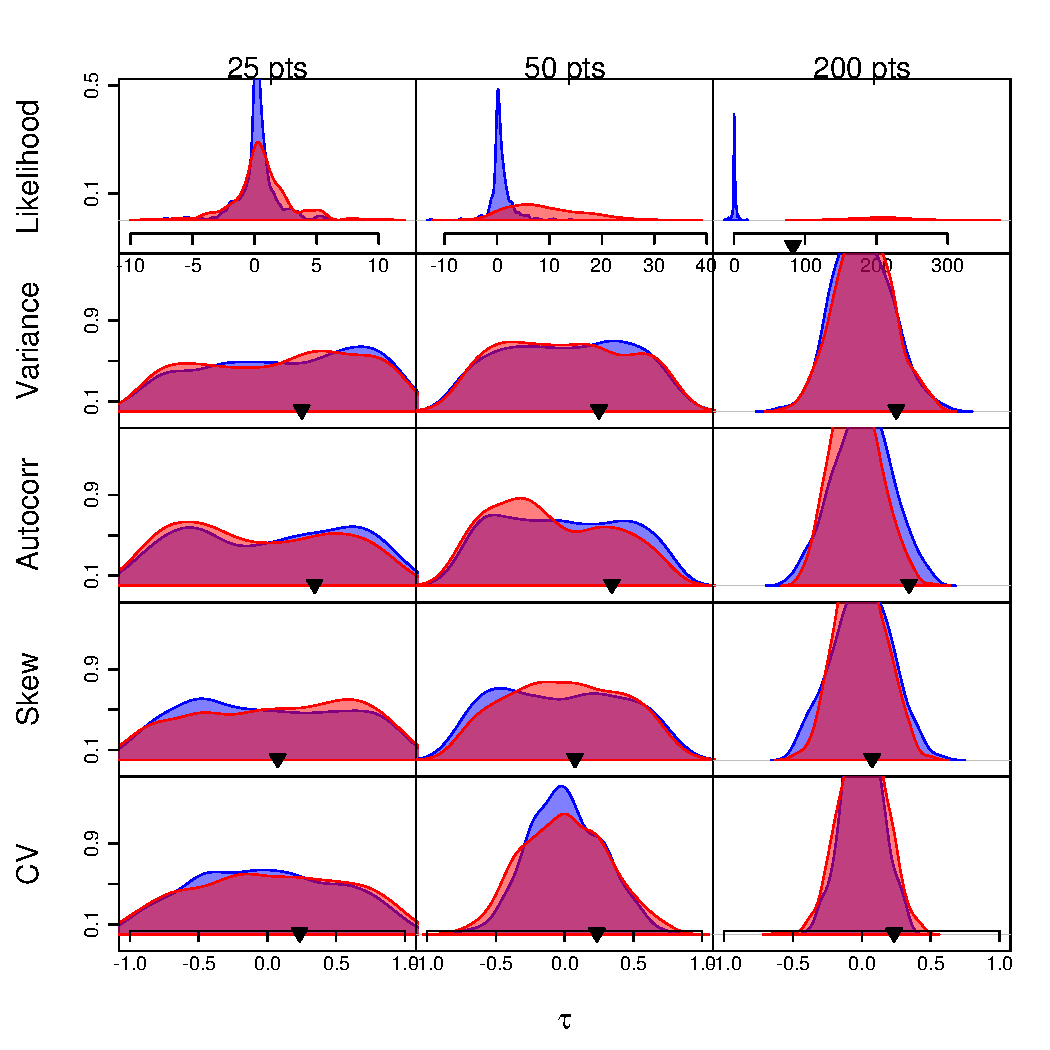
\includegraphics{FigS5.pdf}
  \end{center}
  \caption{Distributions of the indicator statistic as the sampling effort increases in the Glaciation data, corresponding to the fourth column of Fig. 4, main text.  Distributions as described in caption of Fig~\ref{fig:S1}.}
  \label{fig:S5}
\end{figure}

\pagebreak

\section*{ }%bibliography
 \bibliography{/home/cboettig/Documents/Mendeley/bib/library.bib}

 \end{document}



